\documentclass[12pt,a4paper]{article}
\usepackage[a4paper,top=12mm,bottom=14mm,left=15mm,right=15mm]{geometry}
\usepackage[T1]{fontenc}
\usepackage{amsmath}
\usepackage{amssymb}
\usepackage{cancel}
\usepackage{enumitem}
\usepackage{multicol}
\usepackage{array}
\usepackage{xcolor}
\usepackage{tikz}
\usepackage[most]{tcolorbox}
\usetikzlibrary{arrows.meta}

% ================================================================
% Answer key to "Indices and Roots".
%
% This is the worksheet itself with every answer written into its
% answer space, so that a pupil can hold their own sheet beside it and
% check each answer in the place where they wrote it. The teaching
% text, the boxes, the diagrams, the wording of every question and all
% of the \newpage commands are copied from the worksheet unchanged, so
% the two sheets line up page for page. Only the answers are added, and
% no working is shown: the working is in the worked solutions.
%
% Every answer is written in one dark red, the colour set as "answer"
% below, in the same font as the sheet, so that it stands apart from
% the printed question. An answer line is drawn exactly where the
% worksheet draws it and the answer is written on it, with a fraction
% raised so that it sits on the line rather than across it. Where a
% fraction follows an equals sign in a line of maths, the line is drawn
% under the fraction instead, so that the fraction stays level with the
% equals sign. A dotted box keeps its outline with the number written
% inside. Where a question has only blank working space, or a list of
% expressions ending in an equals sign, the answer is written beside
% each expression. The two match-ups are answered by drawing the
% joining lines in the answer colour, and the empty cells of the two
% tables are filled in. The open ended parts are given one short model
% answer, taken from the Answers page and shortened where needed so
% that it fits on the lines the worksheet gives it. The Answers page is
% kept at the back unchanged.
%
% Only text and thin lines are coloured, and no area is filled, so the
% answer key costs no more toner to print than the worksheet.
% ================================================================

\pagestyle{empty}
\linespread{1.15}\selectfont
\setlength{\parskip}{5pt}
\setlist[enumerate,1]{label=\textbf{Q\arabic*.}, leftmargin=*, itemsep=10pt, topsep=6pt, parsep=4pt}
\setlist[enumerate,2]{label=(\alph*), leftmargin=*, itemsep=8pt, topsep=5pt, parsep=3pt}
\setlength{\multicolsep}{4pt}
\setlength{\parindent}{0pt}

\newcommand{\ansline}[1][2.2cm]{\underline{\hspace{#1}}}
% A short gap for a single number, sized to sit inside a line of maths.
\newcommand{\gap}{\underline{\hspace{0.7cm}}}
% A gap for a number that is written as an index, or on the top or the
% bottom of a fraction. An underline sits too low to be read as an
% index, so a faint dotted box marks where the number is written. The
% size is given in points so that the box does not shrink away when it
% is set as an index.
\newcommand{\boxgap}[1][9pt]{\tikz[baseline=-0.8pt]\draw[gray!60,densely dotted,thick]
  (0,0) rectangle (#1,#1);}

% ----------------------------------------------------------------
% The answers. Every answer is written in this colour.
\definecolor{answer}{RGB}{176,24,24}
\newcommand{\ans}[1]{\textcolor{answer}{#1}}
% An answer written on an answer line: \ansfill[<width>][<l|c|r>]{<answer>}.
% The line is the \ansline it replaces, drawn in the same place, and the
% answer is written over it without taking up any height, so the page is
% laid out exactly as the worksheet is. An answer that reaches well below
% the line, such as a fraction, is raised until it sits on the line.
% \ansfill* instead draws the line under the whole answer, for a fraction
% that has to stay level with the equals sign in front of it.
% An answer wider than its line is reported in the log.
\newsavebox{\ansbox}
\newlength{\ansraise}
\NewDocumentCommand{\ansfill}{s O{2.2cm} O{c} +m}{%
  \sbox{\ansbox}{\color{answer}#4}%
  \ifdim\wd\ansbox>#2\relax
    \typeout{ANSWER TOO WIDE on line \the\inputlineno:
      \the\wd\ansbox\space for a line of #2}%
  \fi
  \IfBooleanTF{#1}%
    {\underline{\makebox[#2][#3]{\usebox{\ansbox}}}}%
    {\ifdim\dp\ansbox>4pt\relax
       \setlength{\ansraise}{\dp\ansbox}\addtolength{\ansraise}{0.5pt}%
     \else
       \setlength{\ansraise}{0pt}%
     \fi
     \mbox{\rlap{\ansline[#2]}\makebox[#2][#3]{%
       \raisebox{\ansraise}[0pt][0pt]{\usebox{\ansbox}}}}}}
% A dotted gap with the answer written inside it: \boxans[<size>]{<answer>}.
% The box is drawn exactly as \boxgap draws it, and the answer is set in
% the size of the maths around it, so an index is written as an index.
\makeatletter
\newcommand{\boxans}[2][9pt]{\def\bx@size{#1}\mathpalette\bx@ans{#2}}
\newcommand{\bx@ans}[2]{\tikz[baseline=-0.8pt]{%
  \draw[gray!60,densely dotted,thick] (0,0) rectangle (\bx@size,\bx@size);
  \node[inner sep=0pt,text=answer] at (0.5*\bx@size,0.5*\bx@size) {$\m@th#1#2$};}}
\makeatother
% "= answer", written beside an expression inside maths.
\newcommand{\eqans}[1]{\mathrel{\textcolor{answer}{=}}\textcolor{answer}{#1}}

% A worked example: the method shown in full before it is practised.
% The boxes are tinted only faintly, and their title bars are pale with
% coloured text rather than solid, so that the sheet is cheap to print.
\newtcolorbox{wex}[1]{colback=blue!1,colframe=blue!45!black,boxrule=0.6pt,
  colbacktitle=blue!8,coltitle=blue!50!black,
  left=6pt,right=6pt,top=4pt,bottom=5pt,
  title={\bfseries\small Worked example: #1},fonttitle=\small,
  toptitle=1pt,bottomtitle=1pt}

% The idea a section is built on, stated once and boxed.
\newtcolorbox{keyidea}{colback=orange!2,colframe=orange!60!black,boxrule=0.6pt,
  left=6pt,right=6pt,top=4pt,bottom=4pt}

% The notation for a section, set out so that it can be found again
% from anywhere on the sheet.
\newtcolorbox{notation}[1]{colback=green!1,colframe=green!35!black,boxrule=0.9pt,
  colbacktitle=green!10,coltitle=green!30!black,
  left=8pt,right=8pt,top=5pt,bottom=5pt,
  title={\bfseries Notation: #1},fonttitle=\normalsize,
  toptitle=2pt,bottomtitle=2pt}

% A warning about a mistake that is easy to make.
\newtcolorbox{warning}{colback=red!2,colframe=red!55!black,boxrule=0.6pt,
  left=6pt,right=6pt,top=4pt,bottom=4pt}

% The section headings, kept tight so the parts do not eat the page.
\newcommand{\heading}[1]{%
  \vspace{2pt}
  {\color{blue!45!black}\rule{\linewidth}{1pt}}\\[1pt]
  {\large\bfseries #1}\\[-6pt]
  {\color{blue!45!black}\rule{\linewidth}{0.4pt}}
  \vspace{2pt}}
\newcommand{\parttitle}[2]{\heading{Part #1: #2}}

% ----------------------------------------------------------------
% A match-up: calculations in a numbered column on the left, answers in
% a lettered column on the right, with a gap between them for the lines
% pupils draw. The answers are deliberately out of order.
% \matchup[<row spacing>][<column gap>]{<left items>}{<right items>}[<joins>]
% Each item is written inside braces so that it counts as one item.
% In the answer key the joins are listed as <number>/<letter>, for
% example [1/D,2/H], and each join is drawn as a line in the answer
% colour from the numbered box to the lettered box.
\newcommand{\mletter}[1]{\ifcase\numexpr#1\relax\or A\or B\or C\or D\or E\or
  F\or G\or H\or I\or J\fi}
% The position in the right-hand column of a letter, so that D gives 4.
\newcommand{\mnumber}[1]{\if A#11\fi\if B#12\fi\if C#13\fi\if D#14\fi
  \if E#15\fi\if F#16\fi\if G#17\fi\if H#18\fi\if I#19\fi\if J#110\fi}
\NewDocumentCommand{\matchup}{O{1.1} O{7.2} +m +m O{}}{%
\par\vspace{2pt}\noindent\hfil
\begin{tikzpicture}[mbox/.style={draw=blue!45!black,rounded corners=3pt,thick,
    fill=white,minimum width=2.9cm,minimum height=0.9cm,inner sep=3pt}]
  \foreach [count=\i from 1] \l in {#3} {%
    \node[mbox] (mL\i) at (0,{-#1*\i}) {\l};
    \node[font=\small\bfseries,anchor=east] at ([xshift=-5pt]mL\i.west) {\i.};}
  \foreach [count=\j from 1] \r in {#4} {%
    \node[mbox] (mR\j) at (#2,{-#1*\j}) {\r};
    \node[font=\small\bfseries,anchor=west] at ([xshift=5pt]mR\j.east) {\mletter{\j}};}
  \if\relax\detokenize{#5}\relax\else
    \foreach \p/\q in {#5} {%
      \edef\mright{\mnumber{\q}}%
      \draw[answer,line width=0.9pt] (mL\p.east) -- (mR\mright.west);}
  \fi
\end{tikzpicture}%
\hfil\par\vspace{2pt}}

% ----------------------------------------------------------------
% A 3 by 3 grid of unit squares, which is what 3 squared counts.
\newcommand{\squarepic}{%
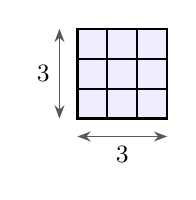
\begin{tikzpicture}[scale=0.38]
  \foreach \x in {0,1,2} \foreach \y in {0,1,2}
    \draw[thick,fill=blue!7] (\x,\y) rectangle ++(1,1);
  \draw[<->,>=Stealth,gray!70!black] (0,-0.6) -- (3,-0.6)
    node[midway,below,font=\small,black] {$3$};
  \draw[<->,>=Stealth,gray!70!black] (-0.6,0) -- (-0.6,3)
    node[midway,left,font=\small,black] {$3$};
\end{tikzpicture}}

% A cube of side 2, divided into the 8 unit cubes that 2 cubed counts.
\newcommand{\cubepic}{%
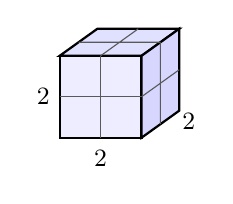
\begin{tikzpicture}[scale=0.52,x={(1cm,0cm)},y={(0.46cm,0.33cm)},z={(0cm,1cm)}]
  \draw[thick,fill=blue!7]  (0,0,0)--(2,0,0)--(2,0,2)--(0,0,2)--cycle;
  \draw[thick,fill=blue!12] (0,0,2)--(2,0,2)--(2,2,2)--(0,2,2)--cycle;
  \draw[thick,fill=blue!16] (2,0,0)--(2,2,0)--(2,2,2)--(2,0,2)--cycle;
  \draw[gray!70!black] (1,0,0)--(1,0,2) (0,0,1)--(2,0,1);
  \draw[gray!70!black] (1,0,2)--(1,2,2) (0,1,2)--(2,1,2);
  \draw[gray!70!black] (2,1,0)--(2,1,2) (2,0,1)--(2,2,1);
  \node[font=\small] at (1,0,-0.5) {$2$};
  \node[font=\small] at (-0.4,0,1) {$2$};
  \node[font=\small] at (2.6,1.2,0) {$2$};
\end{tikzpicture}}

% ----------------------------------------------------------------
% The shapes of the first four dimensions, each drawn with a dot on
% every corner so that the corners can be counted from the picture.
% The dot radius is given in points, so it stays the same size however
% the picture is scaled.
\newcommand{\pointpic}[2]{%
\begin{tikzpicture}[scale=#1]
  \fill[blue!45!black] (0,0) circle (#2);
\end{tikzpicture}}
\newcommand{\linepic}[2]{%
\begin{tikzpicture}[scale=#1]
  \draw[blue!45!black,thick] (0,0)--(2,0);
  \fill[blue!45!black] (0,0) circle (#2) (2,0) circle (#2);
\end{tikzpicture}}
\newcommand{\squarecorners}[2]{%
\begin{tikzpicture}[scale=#1]
  \draw[blue!45!black,thick] (0,0) rectangle (2,2);
  \foreach \a in {0,2} \foreach \b in {0,2} \fill[blue!45!black] (\a,\b) circle (#2);
\end{tikzpicture}}
\newcommand{\cubecorners}[2]{%
\begin{tikzpicture}[scale=#1,x={(1cm,0cm)},y={(0.5cm,0.36cm)},z={(0cm,1cm)},
    line join=round]
  \draw[blue!45!black,thick] (0,0,0)--(2,0,0)--(2,2,0)--(0,2,0)--cycle;
  \draw[blue!45!black,thick] (0,0,2)--(2,0,2)--(2,2,2)--(0,2,2)--cycle;
  \draw[blue!45!black,thick] (0,0,0)--(0,0,2) (2,0,0)--(2,0,2)
    (2,2,0)--(2,2,2) (0,2,0)--(0,2,2);
  \foreach \a in {0,2} \foreach \b in {0,2} \foreach \c in {0,2}
    \fill[blue!45!black] (\a,\b,\c) circle (#2);
\end{tikzpicture}}

% A tesseract, drawn the way a cube is drawn on paper: a small cube
% inside a large cube, with every corner of one joined to the matching
% corner of the other. In four dimensions all eight cubes in the
% picture are the same size and all the joining lines are the same
% length, so the picture stretches the shape in the same way that a
% drawing of a cube stretches its square faces.
\newcommand{\tesspic}[2]{%
\begin{tikzpicture}[scale=#1,x={(1cm,0cm)},y={(0.5cm,0.36cm)},z={(0cm,1cm)},
    line join=round]
  \foreach \a in {0,4} \foreach \b in {0,4} \foreach \c in {0,4}
    \draw[gray!55] (\a,\b,\c) -- ({1+\a/2},{1+\b/2},{1+\c/2});
  \draw[orange!65!black,thick] (1,1,1)--(3,1,1)--(3,3,1)--(1,3,1)--cycle;
  \draw[orange!65!black,thick] (1,1,3)--(3,1,3)--(3,3,3)--(1,3,3)--cycle;
  \draw[orange!65!black,thick] (1,1,1)--(1,1,3) (3,1,1)--(3,1,3)
    (3,3,1)--(3,3,3) (1,3,1)--(1,3,3);
  \draw[blue!45!black,thick] (0,0,0)--(4,0,0)--(4,4,0)--(0,4,0)--cycle;
  \draw[blue!45!black,thick] (0,0,4)--(4,0,4)--(4,4,4)--(0,4,4)--cycle;
  \draw[blue!45!black,thick] (0,0,0)--(0,0,4) (4,0,0)--(4,0,4)
    (4,4,0)--(4,4,4) (0,4,0)--(0,4,4);
  \foreach \a in {0,4} \foreach \b in {0,4} \foreach \c in {0,4} {%
    \fill[blue!45!black] (\a,\b,\c) circle (#2);
    \fill[orange!65!black] ({1+\a/2},{1+\b/2},{1+\c/2}) circle (#2);}
\end{tikzpicture}}

\begin{document}

\begin{center}
  {\Large\bfseries Indices and Roots --- Answer Key}\\[2pt]
\end{center}

\begin{keyidea}
An \textbf{index} tells us how many times a number is multiplied by itself. So $5^3$ means $5\times5\times5$. The plural
of index is \textbf{indices}. A \textbf{root} undoes an index.
\end{keyidea}

\parttitle{1}{Indices and roots of numbers}

\begin{minipage}[t]{0.56\linewidth}
\vspace{0pt}
$3^2$ is read ``three squared''. $2^3$ is read ``two cubed''. 

\vspace{4pt}
The \textbf{square root} of a number is the value that gives that number when it (the square root) is
multiplied by itself, so $\sqrt{9}=3$. The \textbf{cube root} of a number is
the value that gives that number when three of them are multiplied together, so
\mbox{$\sqrt[3]{8}=2$}.
\end{minipage}\hfill
\begin{minipage}[t]{0.41\linewidth}
\vspace{0pt}
\centering
\begin{tabular}{@{}c@{\hspace{0.9em}}c@{}}
\squarepic & \cubepic\\[4pt]
{\small $3^2=3\times3=9$} & {\small $2^3=2\times2\times2=8$}\\
\end{tabular}
\end{minipage}

\vspace{2pt}
\begin{notation}{indices and roots}
\renewcommand{\arraystretch}{1.4}%
\begin{tabular}{@{}>{\large}p{4.3cm}@{\hspace{0.8em}}p{5.0cm}@{\hspace{0.8em}}l@{}}
$a^2=a\times a$ & ``$a$ squared'' & for example \; $7^2=7\times7=49$\\
$a^3=a\times a\times a$ & ``$a$ cubed'' & for example \; $2^3=2\times2\times2=8$\\
$\sqrt{a}$ & the square root of $a$ & for example \; $\sqrt{49}=7$\\
$\sqrt[3]{a}$ & the cube root of $a$ & for example \; $\sqrt[3]{8}=2$\\
\end{tabular}

\vspace{2pt}
An index multiplies the base by itself, and a root finds the base
again.
\end{notation}

\begin{enumerate}

\item Work out each calculation on the left and draw a line joining it to
its answer on the right. Check your answers on a calculator afterwards.
\matchup{{$5^2$},{$\sqrt{100}$},{$2^3$},{$0.2^2$},{$\sqrt{0.25}$},{$10^3$},
  {$\sqrt[3]{8}$},{$1.5^2$}}%
  {{$0.5$},{$8$},{$2$},{$25$},{$1000$},{$0.04$},{$2.25$},{$10$}}%
  [1/D,2/H,3/B,4/F,5/A,6/E,7/C,8/G]

\end{enumerate}

\begin{enumerate}[resume]

\newpage{}

\item The shapes are not drawn to scale.


\begin{enumerate}
  \item A square patio has sides of length $6$ m. Work out its area.

\vspace{2pt}
\begin{minipage}[t]{0.34\linewidth}
\centering
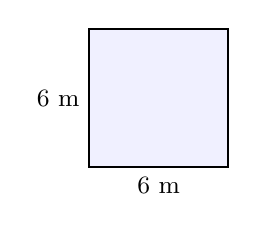
\begin{tikzpicture}[baseline=(current bounding box.north),scale=0.8]
  \draw[thick,fill=blue!6] (0,0) rectangle (2.2,2.2);
  \node[below,font=\small] at (1.1,0) {$6$ m};
  \node[left,font=\small] at (0,1.1) {$6$ m};
\end{tikzpicture}
\end{minipage}%
\begin{minipage}[t]{0.62\linewidth}
\vspace{1.4em}
Area $=6^2=6\times6=\ansfill[1.8cm]{$36$}$ m$^2$
\end{minipage}

  \item A second square patio has an area of $144$ m$^2$. Work out the length
        of one of its sides.

\vspace{2pt}
\begin{minipage}[t]{0.34\linewidth}
\centering
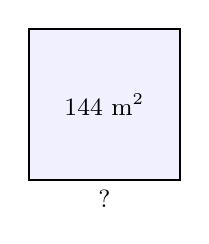
\begin{tikzpicture}[baseline=(current bounding box.north),scale=0.8]
  \draw[thick,fill=blue!6] (0,0) rectangle (2.4,2.4);
  \node[font=\small] at (1.2,1.2) {$144$ m$^2$};
  \node[below,font=\small] at (1.2,0) {$?$};
\end{tikzpicture}
\end{minipage}%
\begin{minipage}[t]{0.62\linewidth}
\vspace{1.4em}
Side $=\sqrt{144}=\ansfill[1.8cm]{$12$}$ m
\end{minipage}

  \item A storage box is a cube with edges of length $4$ cm. Work out its
        volume.

\vspace{2pt}
\begin{minipage}[t]{0.34\linewidth}
\centering
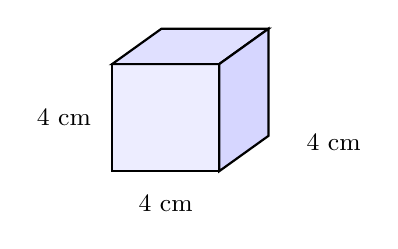
\begin{tikzpicture}[baseline=(current bounding box.north),scale=0.68,
    x={(1cm,0cm)},y={(0.46cm,0.33cm)},z={(0cm,1cm)}]
  \draw[thick,fill=blue!7]  (0,0,0)--(2,0,0)--(2,0,2)--(0,0,2)--cycle;
  \draw[thick,fill=blue!12] (0,0,2)--(2,0,2)--(2,2,2)--(0,2,2)--cycle;
  \draw[thick,fill=blue!16] (2,0,0)--(2,2,0)--(2,2,2)--(2,0,2)--cycle;
  \node[font=\small] at (1,0,-0.6) {$4$ cm};
  \node[font=\small] at (-0.9,0,1) {$4$ cm};
  \node[font=\small] at (3.4,1.6,0) {$4$ cm};
\end{tikzpicture}
\end{minipage}%
\begin{minipage}[t]{0.62\linewidth}
\vspace{1.4em}
Volume $=4^3=\ansfill[3.4cm]{$64$}$ cm$^3$
\end{minipage}

  \item A second storage box is a cube with a volume of $125$ cm$^3$. Work out
        the length of one of its edges.

\vspace{2pt}
\begin{minipage}[t]{0.34\linewidth}
\centering
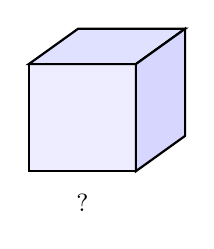
\begin{tikzpicture}[baseline=(current bounding box.north),scale=0.68,
    x={(1cm,0cm)},y={(0.46cm,0.33cm)},z={(0cm,1cm)}]
  \draw[thick,fill=blue!7]  (0,0,0)--(2,0,0)--(2,0,2)--(0,0,2)--cycle;
  \draw[thick,fill=blue!12] (0,0,2)--(2,0,2)--(2,2,2)--(0,2,2)--cycle;
  \draw[thick,fill=blue!16] (2,0,0)--(2,2,0)--(2,2,2)--(2,0,2)--cycle;
  \node[font=\small] at (1,0,-0.6) {$?$};
\end{tikzpicture}

\vspace{1pt}
{\small Volume $=125$ cm$^3$}
\end{minipage}%
\begin{minipage}[t]{0.62\linewidth}
\vspace{1.4em}
Edge $=\ansfill[3.4cm]{$5$}$ cm
\end{minipage}

  \item A square floor tile has an area of $0.25$ m$^2$. Work out the length of
        one of its sides.

\vspace{2pt}
\begin{minipage}[t]{0.34\linewidth}
\centering
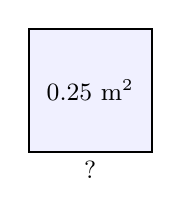
\begin{tikzpicture}[baseline=(current bounding box.north),scale=0.8]
  \draw[thick,fill=blue!6] (0,0) rectangle (1.95,1.95);
  \node[font=\small] at (0.975,0.975) {$0.25$ m$^2$};
  \node[below,font=\small] at (0.975,0) {$?$};
\end{tikzpicture}
\end{minipage}%
\begin{minipage}[t]{0.62\linewidth}
\vspace{1.4em}
Side $=\sqrt{0.25}=\ansfill[1.8cm]{$0.5$}$ m
\end{minipage}

  \item A square garden has an area of $50$ m$^2$. Without a calculator, find
        the two whole numbers that the length of one side lies between. Explain
        how you know.

\vspace{2pt}
\begin{minipage}[t]{0.34\linewidth}
\centering
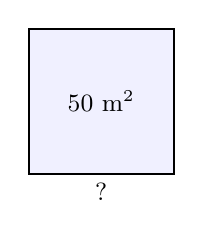
\begin{tikzpicture}[baseline=(current bounding box.north),scale=0.8]
  \draw[thick,fill=blue!6] (0,0) rectangle (2.3,2.3);
  \node[font=\small] at (1.15,1.15) {$50$ m$^2$};
  \node[below,font=\small] at (1.15,0) {$?$};
\end{tikzpicture}
\end{minipage}%
\begin{minipage}[t]{0.62\linewidth}
\vspace{1.4em}
The side is between \ansfill[1.2cm]{$7$} m and \ansfill[1.2cm]{$8$} m, because

\vspace{14pt}
\ansfill[9.5cm][l]{$7^2=49$ and $8^2=64$, and $50$ is between $49$ and $64$.}
\end{minipage}
\end{enumerate}

\end{enumerate}

\vspace{6pt}

\newpage{}

\parttitle{2}{Indices and algebraic variables}

An \textbf{algebraic variable}, such as $a$, $x$ or $m$, could be any number. Just like $5^3=5\times5\times5$, $a^3$ means $a\times a\times a$.


\begin{warning}
In $5a^2$ the index belongs to the $a$ only, so $5a^2=5\times a\times a$. It is
\textbf{not} $5a\times5a$. If $a=2$ then $5a^2=5\times2\times2=20$, but
$5a\times5a=10\times10=100$.
\end{warning}

\begin{wex}{writing a fraction in index form}
\small
Write $\dfrac{a\times a\times a}{b\times b}$ in index form.

\smallskip
\renewcommand{\arraystretch}{1.6}
\begin{tabular}{@{}l@{\hspace{1.2em}}l@{}}
\textbf{Step 1 --- count the numerator.}
  & $a$ appears $3$ times, so the numerator is $a^3$.\\
\textbf{Step 2 --- count the denominator.}
  & $b$ appears $2$ times, so the denominator is $b^2$.\\
\textbf{Step 3 --- write the fraction.}
  & $\dfrac{a\times a\times a}{b\times b}=\dfrac{a^3}{b^2}$\\
\end{tabular}
\end{wex}


\begin{enumerate}[resume]

\item Write each expression in index form. Fill in the gaps in parts (a) and
(b), then simplify the remaining expressions in the same way.
\begin{enumerate}
  \item $a\times a\times a\times a=a^{\boxans{4}}$
  \item $\dfrac{c\times c\times c}{d\times d}=\dfrac{c^{\boxans[7pt]{3}}}{d^{\boxans[7pt]{2}}}$
\end{enumerate}
\vspace{4pt}
\begin{multicols}{3}
\begin{enumerate}[resume]
  \item $b\times b\times b\times b\times b\eqans{b^5}$
  \item $3\times m\times m\eqans{3m^2}$
  \item $\dfrac{p\times p\times p}{q\times q\times q\times q}\eqans{\dfrac{p^3}{q^4}}$
  \item $\dfrac{2\times x\times x\times x}{y\times y}\eqans{\dfrac{2x^3}{y^2}}$
  \item $\dfrac{a\times a\times b\times b\times b}{c\times c}\eqans{\dfrac{a^2b^3}{c^2}}$
  \item $\dfrac{t\times t}{5\times u\times u\times u}\eqans{\dfrac{t^2}{5u^3}}$
\end{enumerate}
\end{multicols}
\vspace{8em}

\item Write each expression out in full as a multiplication. The first one is
done for you.
\begin{enumerate}
  \item $x^3=x\times x\times x$
\end{enumerate}
\vspace{2pt}
\begin{multicols}{2}
\begin{enumerate}[resume]
  \item $y^5=\ansfill[4cm]{$y\times y\times y\times y\times y$}$
  \item $4t^2=\ansfill[4cm]{$4\times t\times t$}$
  \item $\dfrac{m^2}{n^3}=\ansfill*[4cm]{$\dfrac{m\times m}{n\times n\times n}$}$
  \item $\dfrac{a^4}{b}=\ansfill*[4cm]{$\dfrac{a\times a\times a\times a}{b}$}$
\end{enumerate}
\end{multicols}

\end{enumerate}

\vspace{6pt}

\newpage{}

\parttitle{3}{Cancelling factors in a fraction}

A fraction stays the same
value when the numerator and the denominator are both divided by the same
number. Since the new fraction is \textbf{equivalent} to the original.

\begin{keyidea}
When the numerator and the denominator are written as multiplications, a factor
that appears in both can be divided out of both. This is called
\textbf{cancelling}, and it is written by crossing the factor out on the top
and on the bottom.
\end{keyidea}

\begin{wex}{simplify $\dfrac{12}{18}$}
\small
\renewcommand{\arraystretch}{1.9}
\begin{tabular}{@{}l@{\hspace{1.2em}}l@{}}
\textbf{Step 1 --- write the numerator and the denominator as multiplications.}
  & $\dfrac{12}{18}=\dfrac{2\times2\times3}{2\times3\times3}$\\
\textbf{Step 2 --- cross out each factor that appears in both.}
  & $\dfrac{12}{18}=\dfrac{\cancel{2}\times2\times\cancel{3}}
    {\cancel{2}\times\cancel{3}\times3}$\\
\textbf{Step 3 --- multiply what is left on the top and on the bottom.}
  & $\dfrac{12}{18}=\dfrac{2}{3}$\\
\end{tabular}
\end{wex}

\begin{enumerate}[resume]

\item Simplify each fraction by cancelling. Fill in the gaps in parts (a) and
(b), then do parts (c) to (f) in the same way.
\begin{enumerate}
  \item $\dfrac{8}{12}=\dfrac{2\times2\times2}{2\times2\times3}
         =\dfrac{\cancel{2}\times\cancel{2}\times2}
          {\cancel{2}\times\cancel{2}\times3}
         =\dfrac{\boxans[11pt]{2}}{\boxans[11pt]{3}}$
  \item $\dfrac{15}{25}=\dfrac{5\times3}{5\times\boxans[11pt]{5}}
         =\dfrac{\boxans[11pt]{3}}{\boxans[11pt]{5}}$
\end{enumerate}
\vspace{6pt}
\begin{multicols}{4}
\begin{enumerate}[resume]
  \item $\dfrac{18}{24}\eqans{\dfrac{3}{4}}$
  \item $\dfrac{14}{21}\eqans{\dfrac{2}{3}}$
  \item $\dfrac{45}{60}\eqans{\dfrac{3}{4}}$
  \item $\dfrac{24}{36}\eqans{\dfrac{2}{3}}$
\end{enumerate}
\end{multicols}
\vspace{6em}

% The list inside multicols does not pass its count on, so the letters
% after (f) are started by hand.
\begin{enumerate}[start=7]
  \item $12$ of the $28$ pupils in a class walk to school. The picture shows
        the class, with the pupils who walk shaded. Write the fraction of the
        class who walk to school in its simplest form.

\vspace{4pt}
\begin{minipage}[t]{0.40\linewidth}
\centering
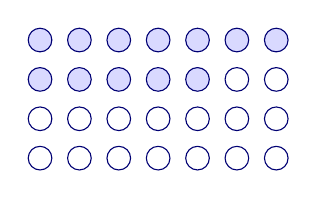
\begin{tikzpicture}[baseline=(current bounding box.north),scale=0.5]
  \foreach \i in {0,...,27} {
    \pgfmathtruncatemacro{\col}{mod(\i,7)}
    \pgfmathtruncatemacro{\row}{\i/7}
    \ifnum\i<12
      \draw[blue!45!black,fill=blue!15] (\col,-\row) circle (0.3);
    \else
      \draw[blue!45!black,fill=white] (\col,-\row) circle (0.3);
    \fi}
\end{tikzpicture}
\end{minipage}%
\begin{minipage}[t]{0.56\linewidth}
\vspace{0.6em}
Fraction who walk $=\dfrac{12}{28}=\ansfill*[3cm]{$\dfrac{3}{7}$}$
\end{minipage}

\vspace{3em}
  \item A cake mixture weighs $120$ g, and $45$ g of it is sugar. Write the
        fraction of the mixture that is sugar in its simplest form.

\vspace{6pt}
\ans{$\dfrac{45}{120}=\dfrac{3}{8}$}

\vspace{5em}
\end{enumerate}

\end{enumerate}


\newpage{}

Algebraic variables cancel in the same way as numbers. When every factor on the bottom cancels, the denominator
is $1$, not nothing, a fraction with a denominator of $1$ is equal to its
numerator.

\begin{wex}{cancelling with numbers and variables}
\small
\renewcommand{\arraystretch}{2.2}
\begin{tabular}{@{}l@{\hspace{1.5em}}l@{}}
$\dfrac{a\times a\times a}{a\times a}
  =\dfrac{\cancel{a}\times\cancel{a}\times a}{\cancel{a}\times\cancel{a}}
  =\dfrac{a}{1}=a$
  & every factor on the bottom cancels, leaving $1$\\
$\dfrac{2\times3\times a\times a}{2\times a}
  =\dfrac{\cancel{2}\times3\times\cancel{a}\times a}
   {\cancel{2}\times\cancel{a}}=\dfrac{3\times a}{1}=3a$
  & the numbers and the variables are cancelled separately\\
\end{tabular}
\end{wex}

\begin{enumerate}[resume]

\item Simplify each fraction by cancelling, then write the answer in index
form. Fill in the gaps in part (a) first.
\begin{enumerate}
  \item $\dfrac{a\times a\times a\times a}{a\times a}
         =\dfrac{\cancel{a}\times\cancel{a}\times a\times a}
          {\cancel{a}\times\cancel{a}}=\dfrac{a\times a}{1}=a^{\boxans{2}}$
\end{enumerate}
\vspace{6pt}
\begin{enumerate}[resume]
  \item $\dfrac{b\times b\times b\times b\times b}{b\times b} =\ans{b^3}$
  \item $\dfrac{2\times2\times m\times m}{2\times m}=\ans{2m}$
  \item $\dfrac{3\times5\times p\times p\times p}{5\times p}=\ans{3p^2}$
  \item $\dfrac{x\times x\times y}{x\times y\times y}=\ans{\dfrac{x}{y}}$
  \item $\dfrac{2\times3\times t\times t}{3\times3\times t}=\ans{\dfrac{2t}{3}}$
  \item $\dfrac{4\times x\times x\times y}{6\times x\times y\times y}=\ans{\dfrac{2x}{3y}}$
  \item $\dfrac{5\times5\times a\times b\times b}{5\times a\times a\times b}=\ans{\dfrac{5b}{a}}$
  \item Lena simplifies $\dfrac{a\times a}{a\times a\times a}$ and writes $a$.
        Explain the mistake Lena has made, and write down the correct answer.

\vspace{6pt}
\ansfill[16cm][l]{Two $a$s cancel from the numerator and the denominator. This
  leaves $1$ in the numerator}

\vspace{16pt}
\ansfill*[16cm][l]{and one $a$ in the denominator, not in the numerator. The
  correct answer is $\dfrac{1}{a}$.}
\end{enumerate}
\vspace{10em}

\end{enumerate}

\newpage{}

\parttitle{4}{Simplifying fractions written with indices}

A fraction written with indices is simplified in the same way. We write each
power out in full as a multiplication, cancel the factors that appear on the
top and on the bottom, and write what is left in index form.

\begin{wex}{simplifying fractions written with indices}
\small
\renewcommand{\arraystretch}{2.2}
\begin{tabular}{@{}l@{\hspace{2em}}l@{}}
$\dfrac{a^5}{a^2}
  =\dfrac{\cancel{a}\times\cancel{a}\times a\times a\times a}
   {\cancel{a}\times\cancel{a}}=a^3$
  & two of the five $a$s cancel, leaving three\\
$\dfrac{6a^3}{2a}
  =\dfrac{\cancel{2}\times3\times\cancel{a}\times a\times a}
   {\cancel{2}\times\cancel{a}}=3a^2$
  & $6=2\times3$, so a factor of $2$ cancels as well\\
\end{tabular}
\end{wex}

\begin{enumerate}[resume]

\item Simplify each fraction on the left. Draw a line joining it to its answer
on the right.

\vspace{4pt}
\matchup[1.6]{{$\dfrac{a^5}{a^2}$},{$\dfrac{a^2}{a^2}$},{$\dfrac{6a^4}{2a^2}$},
  {$\dfrac{a^3b}{ab}$},{$\dfrac{4a^2}{8a}$},{$\dfrac{a^2b^3}{a^2b}$},
  {$\dfrac{10a^3}{5a^3}$},{$\dfrac{a^6}{a^2}$}}%
  {{$b^2$},{$a^4$},{$2$},{$a^3$},{$\dfrac{a}{2}$},{$1$},{$a^2$},{$3a^2$}}%
  [1/D,2/F,3/H,4/G,5/E,6/A,7/C,8/B]

\end{enumerate}

\newpage

\begin{enumerate}[resume]

\item
\begin{enumerate}
  \item Write down three different fractions that simplify to $2a^2$. One of
        them must have a number other than $1$ in the denominator.

\vspace{12pt}
\ansfill[3.4cm]{$\dfrac{2a^3}{a}$}\hfill \ansfill[3.4cm]{$\dfrac{4a^3}{2a}$}\hfill
\ansfill[3.4cm]{$\dfrac{6a^5}{3a^3}$}

\vspace{12pt}
  \item Write down a fraction (not equal to $\frac{a^2}{b}$) using the variables $a$ and $b$ that simplifies
        to $\frac{a^2}{b}$.

\vspace{16pt}
\ansfill[5cm]{$\dfrac{a^3}{ab}$}


\vspace{8pt}
\item Write down a fraction using the variables $x$, $y$ and $z$ that simplifies to
      $\frac{1}{xy^2}$.

\vspace{16pt}
\ansfill[5cm]{$\dfrac{z}{xy^2z}$}


\vspace{8pt}
  \item Ben says that $\frac{3a^2}{3a^2}=0$, because every factor on the top
        and on the bottom cancels and nothing is left. Explain the mistake Ben
        has made, and write down the correct answer.

\vspace{6pt}
\ansfill[16cm][l]{Cancelling divides the numerator and the denominator by the
  same factor, and a}

\vspace{16pt}
\ansfill[16cm][l]{number divided by itself is $1$, not $0$. So
  $3a^2\div3a^2=1$, and the correct answer is $1$.}
\end{enumerate}

\item In this question we find a quicker way to simplify a fraction such as
$\dfrac{a^7}{a^3}$.
\begin{enumerate}
  \item Simplify each fraction by writing it out in full and cancelling. Give
        each answer in index form.

\vspace{8pt}
$\dfrac{a^7}{a^3}=\ansfill[2.4cm]{$a^4$}$ \hfill $\dfrac{b^9}{b^4}=\ansfill[2.4cm]{$b^5$}$
\hfill $\dfrac{c^6}{c^5}=\ansfill[2.4cm]{$c$}$

\vspace{3.5em}
  \item Look at the indices in each fraction and in its answer. Describe a
        quicker way to find the answer without writing the powers out in full.

\vspace{6pt}
\ansfill[16cm][l]{We subtract the index in the denominator from the index in
  the numerator, and}

\vspace{16pt}
\ansfill[16cm][l]{we keep the same base. For example,
  $a^7\div a^3=a^{7-3}=a^4$.}

\vspace{6pt}
  \item Use your quicker way to simplify these fractions.

\vspace{8pt}
$\dfrac{x^{20}}{x^{13}}=\ansfill[2.4cm]{$x^7$}$ \hspace{3em}
$\dfrac{y^{100}}{y^{99}}=\ansfill[2.4cm]{$y$}$

\vspace{6pt}
  \item Use your quicker way on $\dfrac{a^3}{a^3}$. Cancelling shows that
        $\dfrac{a^3}{a^3}=1$. What does this suggest $a^0$ is equal to?

\vspace{10pt}
$\dfrac{a^3}{a^3}=a^{\boxans{0}}$ \hspace{3em} so \hspace{3em} $a^0=\ansfill[2.4cm]{$1$}$
\end{enumerate}

\end{enumerate}

\newpage{}

\vspace{6pt}

\parttitle{5}{Extension: factorials, negative numbers and the fourth dimension}

The \textbf{factorial} of a whole number is written with an exclamation mark
after it. The expression $n!$ means multiply together every whole number from
$n$ down to $1$, so $5!=5\times4\times3\times2\times1=120$.

$10!=10\times9\times8\times7\times6\times5\times4\times3\times2\times1=3\,628\,800$.

\begin{enumerate}[resume]

\item Work out each factorial.
\begin{multicols}{4}
\begin{enumerate}
  \item $3!=\ansfill[1.8cm]{$6$}$
  \item $4!=\ansfill[1.8cm]{$24$}$
  \item $6!=\ansfill[1.8cm]{$720$}$
  \item $1!=\ansfill[1.8cm]{$1$}$
\end{enumerate}
\end{multicols}

\end{enumerate}

\begin{wex}{simplify $\dfrac{6!}{4!}$}
\small
Both factorials are written out in full. Every whole number from $4$ downwards
appears on the top and on the bottom, so all of those factors cancel.

\smallskip
\[\frac{6!}{4!}
  =\frac{6\times5\times\cancel{4}\times\cancel{3}\times\cancel{2}\times\cancel{1}}
   {\cancel{4}\times\cancel{3}\times\cancel{2}\times\cancel{1}}
  =6\times5=30\]
\end{wex}

\begin{enumerate}[resume]

\item Simplify each expression by writing the factorials out in full and
cancelling. Do not work the factorials out first.
\begin{multicols}{3}
\begin{enumerate}
  \item $\dfrac{5!}{3!}\eqans{20}$
  \item $\dfrac{10!}{9!}\eqans{10}$
  \item $\dfrac{8!}{6!}\eqans{56}$
  \item $\dfrac{7!}{5!\times2!}\eqans{21}$
  \item $\dfrac{100!}{98!}\eqans{9900}$
  \item $\dfrac{12!}{10!\times2!}\eqans{66}$
\end{enumerate}
\end{multicols}
\vspace{9em}

\item For any whole number $n$ that is greater than $1$, the expression
$\dfrac{n!}{(n-1)!}$ always simplifies to $n$. Explain why.

\vspace{6pt}
\ansfill[16cm][l]{$n!=n\times(n-1)\times(n-2)\times\cdots\times1$ \ and \
  $(n-1)!=(n-1)\times(n-2)\times\cdots\times1$.}

\vspace{16pt}
\ansfill[16cm][l]{Every factor of $(n-1)!$ also appears in $n!$, so all of
  those factors cancel.}

\vspace{16pt}
\ansfill[16cm][l]{The only factor left in the numerator is $n$, and the
  denominator is $1$, so the answer is $n$.}

\newpage{}

\item When the base is negative, the brackets show that the whole negative
number is multiplied by itself, so $(-2)^3=(-2)\times(-2)\times(-2)$.
\begin{enumerate}
  \item Complete the table.

\vspace{2pt}
\begin{center}
\renewcommand{\arraystretch}{1.8}
\begin{tabular}{|>{\centering\arraybackslash}p{2.4cm}|>{\centering\arraybackslash}p{6.4cm}|>{\centering\arraybackslash}p{2.4cm}|}
\hline
\textbf{Expression} & \textbf{Written out in full} & \textbf{Answer}\\
\hline
$(-2)^2$ & $(-2)\times(-2)$ & $4$\\ \hline
$(-2)^3$ & $(-2)\times(-2)\times(-2)$ & \ans{$-8$}\\ \hline
$(-2)^4$ & \ans{$(-2)\times(-2)\times(-2)\times(-2)$} & \ans{$16$}\\ \hline
$(-3)^2$ & \ans{$(-3)\times(-3)$} & \ans{$9$}\\ \hline
$(-3)^3$ & \ans{$(-3)\times(-3)\times(-3)$} & \ans{$-27$}\\ \hline
\end{tabular}
\end{center}

  \item Write down what you notice about the sign of the answer when the index
        is even, and when the index is odd.

\vspace{6pt}
\ansfill[16cm][l]{An even index gives a positive answer, and an odd index
  gives a negative answer.}

\vspace{16pt}
  \item Explain why this happens.

\vspace{6pt}
\ansfill[16cm][l]{Each pair of negative factors gives a positive. An odd index
  leaves one negative factor.}
\end{enumerate}

\end{enumerate}


\begin{enumerate}[resume]

\item
\begin{enumerate}
  \item Work out $3\times3$ and $(-3)\times(-3)$. Write down both of the
        numbers that give $9$ when they are multiplied by themselves.

\vspace{8pt}
\ansfill[5.5cm]{$3$} \hspace{1.5em} and \hspace{1.5em} \ansfill[5.5cm]{$-3$}

\vspace{6pt}
The symbol $\sqrt{\phantom{a}}$ means the positive square root only, so
$\sqrt{9}=3$.

\vspace{6pt}
  \item Work out $\sqrt{-9}$ on your calculator. Write down what the calculator
        shows, and explain why.

\vspace{6pt}
\ansfill[16cm][l]{The calculator shows an error. No number multiplied by
  itself gives a negative answer,}

\vspace{16pt}
\ansfill[16cm][l]{because two positive factors or two negative factors
  multiply to give a positive answer.}

\vspace{6pt}
  \item Work out $(-2)\times(-2)\times(-2)$. Use your answer to write down
        $\sqrt[3]{-8}$.

\vspace{8pt}
\ansfill[5.5cm]{$-8$} \hspace{1.5em} so \hspace{1.5em} $\sqrt[3]{-8}=$ \ansfill[3cm]{$-2$}

\vspace{6pt}
  \item Sam says that a root of a negative number can never be found. Use your
        answers to parts (b) and (c) to say whether Sam is right, and explain
        your answer.

\vspace{6pt}
\ansfill[16cm][l]{Sam is not right. A negative number has no square root,
  because an even index always}

\vspace{16pt}
\ansfill[16cm][l]{gives a positive answer. But $\sqrt[3]{-8}=-2$, so a
  negative number does have a cube root.}

\end{enumerate}

\item A square is the two-dimensional shape made by sliding a line at right
angles to itself, a cube is the three-dimensional shape made by sliding a
square at right angles to itself. A \textbf{tesseract} is the shape made by
sliding a cube at right angles to itself, in the fourth direction. There is no
fourth direction in the space we live in, so a tesseract cannot be built, but
it can still be drawn and its measurements can still be worked out.

Below is a drawing of tessaract, or the best we can do in three dimensions. The blue and orange corners would in fact all be the outside of the tesseract, and the fourth lines connecting the inner and outer cubes would form right angles to the remaining lines (we don't have enough dimensions to imagine this!)

\vspace{4pt}
\begin{center}
\tesspic{0.82}{2pt}
\end{center}
\vspace{2pt}

\begin{enumerate}
  \item Complete the table. Count the corners on each picture.
\nopagebreak

\vspace{2pt}
\begin{center}
\renewcommand{\arraystretch}{1.5}
\begin{tabular}{|l|>{\centering\arraybackslash}p{1.6cm}|>{\centering\arraybackslash}p{1.8cm}|>{\centering\arraybackslash}p{1.9cm}|>{\centering\arraybackslash}p{2.0cm}|>{\centering\arraybackslash}p{2.4cm}|}
\hline
\textbf{Shape} & point & line & square & cube & tesseract\\ \hline
\textbf{Picture} & \pointpic{0.4}{3pt} & \linepic{0.45}{3pt}
  & \squarecorners{0.35}{3pt} & \cubecorners{0.35}{3pt}
  & \tesspic{0.28}{1.4pt}\\ \hline
\textbf{Dimensions} & $0$ & $1$ & $2$ & $3$ & $4$\\ \hline
\textbf{Corners} & $1$ & $2$ & $4$ & \ans{$8$} & \ans{$16$}\\ \hline
\end{tabular}
\end{center}

  \item Write the number of corners of the square, the cube and the
        tesseract as a power of $2$.

\vspace{6pt}
Square: \ansfill[2.6cm]{$2^2$} \hfill Cube: \ansfill[2.6cm]{$2^3$} \hfill
Tesseract: \ansfill[2.6cm]{$2^4$}

\vspace{6pt}
  \item The shape after the tesseract has five dimensions. Use the pattern in
        the table to write the number of corners it has as a power of $2$, and
        then work it out.

\vspace{10pt}
Corners $=\ansfill[3cm]{$2^5$}=\ansfill[3cm]{$32$}$

\vspace{6pt}
  \item One of the shapes in this pattern has $1024$ corners. How many
        dimensions does it have? Show how you know.

\vspace{6pt}
\ansfill[16cm][l]{The number of corners is $2$ to the power of the number of
  dimensions.}

\vspace{16pt}
\ansfill[16cm][l]{$1024=2^{10}$, so the shape has $10$ dimensions.}

\newpage{}

\vspace{6pt}
  \item A cube with edges of length $3$ cm has a volume of $3^3=27$ cm$^3$. A
        tesseract with edges of length $3$ cm has a \textbf{hypervolume} of
        $3^4$ cm$^4$. Work out $3^4$.

\vspace{10pt}
$3^4=\ansfill[6cm]{$81$}$ cm$^4$

\vspace{6pt}
  \item A tesseract has a hypervolume of $16$ cm$^4$. The length of one of its
        edges is the \textbf{fourth root} of $16$, written $\sqrt[4]{16}$.
        Work out $\sqrt[4]{16}$ by finding the number that gives $16$ when
        four of them are multiplied together.

\vspace{10pt}
$\sqrt[4]{16}=\ansfill[6cm]{$2$}$ cm

\vspace{6pt}
  \item Show that $(-2)^4=16$ as well. Explain why the edge of the tesseract
        must still be $2$ cm.

\vspace{6pt}
\ansfill[16cm][l]{$(-2)\times(-2)\times(-2)\times(-2)=16$, because the index
  is even.}

\vspace{16pt}
\ansfill[16cm][l]{The edge must still be $2$ cm, because a length cannot be
  negative.}

\vspace{6pt}
  \item A second tesseract has a hypervolume of $81$ cm$^4$. Work out the
        length of one of its edges.

\vspace{10pt}
$\sqrt[4]{81}=\ansfill[6cm]{$3$}$ cm

\vspace{6pt}
  \item A square has $4$ edges, a cube has $12$ edges and a tesseract has $32$
        edges. The $12$ edges of a cube can be written as $3\times2^2$. Write
        the edges of a square and the edges of a tesseract in the same way,
        as a number multiplied by a power of $2$. Then use the pattern to
        predict how many edges the five-dimensional shape has.

\vspace{6pt}
Square: $4=\ansfill[3cm]{$2\times2^1$}$ \hfill Cube: $12=3\times2^2$ \hfill
Tesseract: $32=\ansfill[3cm]{$4\times2^3$}$

\vspace{12pt}
\ansfill[16cm][l]{The number in front is the number of dimensions, and the
  index is one less than it,}

\vspace{16pt}
\ansfill[16cm][l]{so the five-dimensional shape has $5\times2^4=80$ edges.}

\vspace{6pt}
  \item Use both patterns to find the number of corners and the number of edges
        of the six-dimensional shape.

\vspace{10pt}
Corners $=\ansfill[4cm]{$64$}$ \hfill Edges $=\ansfill[4cm]{$192$}$
\end{enumerate}

\end{enumerate}

\newpage

\heading{Answers}

{\small
\begin{multicols}{2}
\raggedcolumns
\setlength{\parskip}{4pt}

\textbf{Q1.} 1--D ($25$) \quad 2--H ($10$) \quad 3--B ($8$) \quad
4--F ($0.04$) \quad 5--A ($0.5$) \quad 6--E ($1000$) \quad 7--C ($2$) \quad
8--G ($2.25$)

\textbf{Q2.} (a) $6\times6=36$ m$^2$ \quad (b) $\sqrt{144}=12$ m \quad
(c) $4\times4\times4=64$ cm$^3$ \quad (d) $\sqrt[3]{125}=5$ cm \quad
(e) $\sqrt{0.25}=0.5$ m \quad (f) Between $7$ m and $8$ m, because
$7^2=49$ and $8^2=64$, and $50$ is between $49$ and $64$.

\textbf{Q3.} (a) $a^4$ \quad (b) $\dfrac{c^3}{d^2}$ \quad (c) $b^5$ \quad
(d) $3m^2$ \quad (e) $\dfrac{p^3}{q^4}$ \quad (f) $\dfrac{2x^3}{y^2}$ \quad
(g) $\dfrac{a^2b^3}{c^2}$ \quad (h) $\dfrac{t^2}{5u^3}$

\textbf{Q4.} (b) $y\times y\times y\times y\times y$ \quad
(c) $4\times t\times t$ \quad (d) $\dfrac{m\times m}{n\times n\times n}$ \quad
(e) $\dfrac{a\times a\times a\times a}{b}$

\textbf{Q5.} (a) $\dfrac{2}{3}$ \quad
(b) $\dfrac{5\times3}{5\times5}=\dfrac{3}{5}$ \quad (c) $\dfrac{3}{4}$ \quad
(d) $\dfrac{2}{3}$ \quad (e) $\dfrac{3}{4}$ \quad (f) $\dfrac{2}{3}$ \quad
(g) $\dfrac{12}{28}=\dfrac{3}{7}$ \quad (h) $\dfrac{45}{120}=\dfrac{3}{8}$

\textbf{Q6.} (a) $a^2$ \quad (b) $b^3$ \quad (c) $2m$ \quad (d) $3p^2$ \quad
(e) $\dfrac{x}{y}$ \quad (f) $\dfrac{2t}{3}$ \quad (g) $\dfrac{2x}{3y}$
\quad (h) $\dfrac{5b}{a}$ \quad (i) Two $a$s cancel from the top and the
bottom, which leaves $1$ on the top and one $a$ on the bottom. Lena has put the
$a$ that is left on the top. The answer is $\dfrac{1}{a}$.

\textbf{Q7.} 1--D ($a^3$) \quad 2--F ($1$) \quad 3--H ($3a^2$) \quad
4--G ($a^2$) \quad 5--E ($\frac{a}{2}$) \quad 6--A ($b^2$) \quad
7--C ($2$) \quad 8--B ($a^4$)

\textbf{Q8.} (a) There are many answers, for example $\dfrac{2a^3}{a}$, \;
$\dfrac{4a^3}{2a}$ \; and \; $\dfrac{6a^5}{3a^3}$. \quad (b) There are many
answers, for example $\dfrac{a^3}{ab}$ or $\dfrac{a^2b}{b^2}$. \quad
(c) There are many answers, for example $\dfrac{z}{xy^2z}$ or
$\dfrac{xz}{x^2y^2z}$. \quad (d) Cancelling divides the top and the bottom by the same factor, and a number
divided by itself is $1$, not $0$. What is left on the top is $1$ and what is
left on the bottom is $1$, so $\dfrac{3a^2}{3a^2}=\dfrac{1}{1}=1$.

\textbf{Q9.} (a) $a^4$, \; $b^5$, \; $c$ \quad (b) Subtract the index on the
bottom from the index on the top, and keep the same base. \quad
(c) $x^7$, \; $y$ \quad (d) $\dfrac{a^3}{a^3}=a^{3-3}=a^0$, and cancelling
gives $1$, so $a^0=1$.

\textbf{Q10.} (a) $6$ \quad (b) $24$ \quad (c) $720$ \quad (d) $1$

\textbf{Q11.} (a) $5\times4=20$ \quad (b) $10$ \quad (c) $8\times7=56$ \quad
(d) $\dfrac{7\times6}{2\times1}=21$ \quad (e) $100\times99=9900$ \quad
(f) $\dfrac{12\times11}{2\times1}=66$

\textbf{Q12.} $n!=n\times(n-1)\times(n-2)\times\cdots\times1$ and
$(n-1)!=(n-1)\times(n-2)\times\cdots\times1$. Every factor of $(n-1)!$ also
appears in $n!$, so all of them cancel. The only factor left on the top is $n$,
and the bottom is $1$.

\textbf{Q13.} (a) $(-2)^3=-8$; \;
$(-2)^4=(-2)\times(-2)\times(-2)\times(-2)=16$; \;
$(-3)^2=(-3)\times(-3)=9$; \; $(-3)^3=(-3)\times(-3)\times(-3)=-27$. \quad
(b) An even index gives a positive answer and an odd index gives a negative
answer. \quad (c) Two negative numbers multiplied together give a positive
answer, so the negative signs pair up. An even index leaves no negative sign
over, and an odd index leaves one negative sign over.

\textbf{Q14.} (a) $3\times3=9$ and $(-3)\times(-3)=9$, so the two numbers are
$3$ and $-3$. \quad (b) The calculator shows an error. No number multiplied by
itself gives a negative answer, because a positive multiplied by a positive is
positive, and a negative multiplied by a negative is also positive. \quad
(c) $(-2)\times(-2)\times(-2)=-8$, so $\sqrt[3]{-8}=-2$. \quad (d) Sam is not
right. A negative number has no square root, because an even index always gives
a positive answer, but it does have a cube root, because an odd index can give
a negative answer.

\textbf{Q15.} (a) The cube has $8$ corners and the tesseract has $16$
corners. \quad (b) Square: $4=2^2$; \; cube: $8=2^3$; \; tesseract:
$16=2^4$. The index is the number of dimensions. \quad
(c) $2^5=32$ corners \quad (d) $1024=2^{10}$, so it has $10$ dimensions. \quad
(e) $3^4=3\times3\times3\times3=81$ cm$^4$ \quad
(f) $\sqrt[4]{16}=2$ cm, because $2\times2\times2\times2=16$. \quad
(g) $(-2)\times(-2)\times(-2)\times(-2)=16$, because the index is even. The
edge must still be $2$ cm, because a length cannot be negative. \quad
(h) $\sqrt[4]{81}=3$ cm, because $3\times3\times3\times3=81$. \quad
(i) Square: $4=2\times2^1$; \; tesseract: $32=4\times2^3$. The number in front
is the number of dimensions and the index is one less than it, so the
five-dimensional shape has $5\times2^4=80$ edges. \quad
(j) Corners $=2^6=64$; \; edges $=6\times2^5=192$.

\end{multicols}
}

\end{document}
